%Events------------------------------------------------------------------
\section{Events}
        
    Agent execution is modeled in terms of events. An event is either an operation that involves (shared) memory access or that constrains the order of execution of multiple events.

    \subsection{Event Types}
    
        Given an agent cluster, an \textit{event set} \set{E} is a collection of all events from the agent event lists. This set is composed of mainly two distinct subsets as follows: 

        \begin{itemize}
            \item \textbf{Shared Memory (\set{SM}) Events}
                
                This set is composed of two sets of events; those that write to shared memory called Write events (\set{W}) and those that read from shared memory called Read events (\set{R}). Events that belong to both Write and Read events are called Read-Modify-Write. 
            
            \item \textbf{Synchronize (\set{S}) Events} 
                These events only restrict the ordering of execution of events by agents. For instance $lock$ and $unlock$ type of events can be categorized under Synchronize events. However, this is not stated in the specification\footnotemark. 
    
                \footnotetext{The features of $Lock$ and $Unlock$ events is actually not something given to the programmer to use in Javascript. They areused to implement the feature $wait$ and  $notify$ that the programmer can use which adheres to the semantics of $futexes$ inLinux. Hence, in the original standard of the model, the distinction between lock and unlock is not made, and it is simplystated as Synchronize Event.}
        \end{itemize}
        
        \begin{figure}[H]
            \centering 
            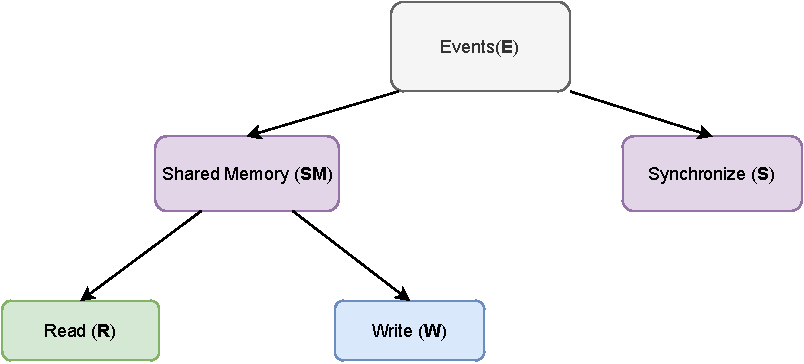
\includegraphics[scale=0.7]{4.ECMAScriptMemoryModel/EventTypes.pdf}
            \caption{Different sets of events.}
        \end{figure}

    %Range of events
    \subsection{Range ($\Re$)}
        Each of the \textit{shared memory events} are associated with a contiguous range of memory on which it operates. Range is a function that maps a shared memory event to the range\footnotemark it operates on. This we represent as a starting index $i$ and a size$s$. So we could represent the range of a write event $w$ as 
                
                \[\Re(w) = (i, s) \]
    
        \footnotetext{The range as per the ECMAScript standard denotes only the set of contiguous byte indices. The starting byte index is kept separate. We find this to be unnecessary. Hence we define range to have starting index and size.}
        
        We define the two binary operators below on ranges: 
        \begin{enumerate}
            \item Intersection $(\cap{_\Re})$ - Set of byte indices common to both ranges.
            \item Union $(\cup_\Re)$ - A unique set of byte indices that exist in both the ranges.  
        \end{enumerate}
        
        Two Ranges can be \textit{disjoint}, \textit{overlapping} or \textit{equal}. We use the binary operators to define these threepossibilities between ranges of events $e$ and $d$ :
        \begin{enumerate}
            \item Disjoint $\Re(e) \cap_\Re \Re(d) = \phi$ 
            \item Overlapping $(\Re(e)\cap_\Re \Re(d) \neq \phi) \wedge (\Re(e) \cap_\Re  \Re(d) \neq \Re(e) \cup_\Re \Re(d))$ - 
            \item Equal $\Re(e) \cap_\Re  \Re(d) = \Re(e) \cup_\Re \Re(d)$ - In simple terms, we define equality as $\Re(e) = \Re(d)$
        \end{enumerate}
            
%Types of Events Based on Order--------------------------------------------------------------------------------------------------------------------
    
    \subsection{Event Order / Event Access Mode} 
        Order signifies the sequence in which event actions are visible to different agents as well as the order in which they are executed by the agents themselves. In our context, there are mainly three types (in C11 memory model, they are called access modes) for each shared memory event that tells us the kind of ordering that it enforces. 
        
        \begin{enumerate}
            \item \textbf{Sequentially Consistent ($sc$)} - Events of this type are \textit{atomic}\footnotemark  in nature. There is a strict global total ordering of such events which is agreed upon by all agents in the agent cluster. 
            
            \item \textbf{Unordered ($uo$)} - Events of this type are considered \textit{non-atomic} and can occur in different orders for each concurrent process. There is no fixed global order respected by agents for such events. 
            
            \item \textbf{Initialize ($init$)} - Events of this type are used to initialize the values in memory before they are accessed by agent events. 
        \end{enumerate}

        All events of type \textit{init} are writes and all Read-Modify-Write events are of type \textit{sc}.  
        We represent the type of events in the memory consistency rules in the format ``$\textit{event} : \textit{type}$''. 
        When representing events in examples, the type would be represented as a subscript: $\textit{event}_\textit{type}$. 
       
        \begin{figure}[H]
            \centering
            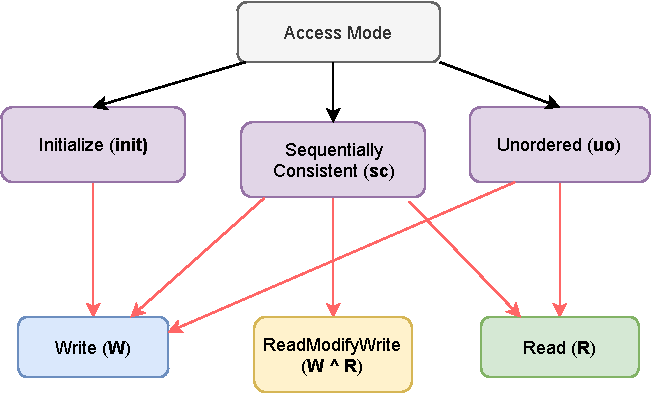
\includegraphics[scale=0.7]{4.ECMAScriptMemoryModel/AccessModes.pdf}
            \caption{Event access modes with its restriction for some events.}
        \end{figure}

        \footnotetext{The word \textit{atomic} does not imply the events are evaluated using just one instruction. For example, a 64-bit sequentially consistent write on a 32-bit system has to be done with two subsequent memory actions. But its intermediate state of write must not be seen by any other agent. In an abstract sense, this event must appear '\textit{atomic}'.The \textit{atomic} here also refers to implications of whether an event's consequence is visible to all other agents in the same global total order or not. The compiler must ensure that for each specific target hardware, such guarantees are satisfied.}

%Tearing factor of events---------------------------------------------------------------------------------------------------------------------------

    \subsection{Tear Free ($tf$) or Tearing $!tf$)}
        Additionally, each shared-memory event is also associated with whether they are tear-free or not. 
        Events that tear are non-aligned accesses requiring more than one memory access. 
        Events that are tear-free are aligned and should appear to be serviced in one memory fetch\footnotemark.

        We represent the tearing of events in the memory consistency rules in the format ``$\textit{event} : \textit{tf/!tf}$''. 
        When representing events in examples, the type would be represented as a subscript: $\textit{event}_\textit{tf/!tf}$. 
       
        \footnotetext{It is not clear whether the alignment is with respect to specific hardware or not. The notion of one memory fetch may not be possible for all hardware practically, but it is something that must appear so. We will see a rule for ensuring this in the memory consistency rules.}
                       